\seccion{Entrop\'ia condicional, informaci\'on mutua, entrop\'ia relativa}
\label{s:SZ:Mutua}

Tratando de un par de variables aleatorias $X$ e $Y$, una cuesti\'on natural que
ocurre  es de  cuantificar la  incerteza que  queda sobre  una de  las variables
cuando se  observa la otra.   Dicho de otra  manera, si se  mide $Y =  y$, ?`que
informaci\'on lleva sobre  $X$? La respuesta a esta  interogaci\'on se encuentra
en la noci\'on de entrop\'ia condicional.  Si uno mide $Y = y$, la descripci\'on
estad\'istica  de $X$  conociendo este  $Y =  y$ se  resuma a  la distribuci\'on
condicional   de  probabilidad  $p_{X|Y}   =  \frac{p_{X,Y}}{p_Y}$.    Con  esta
restricci\'on, se puede evaluar una incerteza sobre $X$, sabiendo que $Y=y$,
%
\[
H(X|Y=y) = H\left( p_{X|Y}(\cdot,y) \right)
\]
%
Entonces, condicionalmente a la variable aleatoria $Y$, la incerteza va a ser el
promedio estad\'istico  sobre todos  los estados $Y$  es decir $H(X|Y)  = \sum_y
p_Y(y) H(X|Y=y)$:
%
\begin{definicion}[Entrop\'ia condicional]\label{def:SZ:entropiacondicional}
  Sean $X$ e  $Y$ dos variables aleatorias discretas,  la entrop\'ia condicional
  de $X$ sabiendo $Y$ es definida por
  %
  \[
  H(X|Y) = - \sum_{x,y} p_{X,Y}(x,y) \log p_{X|Y}(x,y)
  \]
\end{definicion}
%
Esta definici\'on se transpone naturalmente a la entrop\'ia diferencial:
%
\begin{definicion}[Entrop\'ia diferencial condicional]\label{def:SZ:entropiadiferencialcondicional}
  Sean $X$ e  $Y$ dos variables aleatorias continuas,  la entrop\'ia condicional
  de $X$ sabiendo $Y$ es definida por
  %
  \[
  H(X|Y) = - \int_{\Rset^d} p_{X,Y}(x,y) \log p_{X|Y}(x,y) \, dx \, dy
  \]
\end{definicion}

Si $X$ e $Y$ son indepedientes, $p_{X|Y}$ se reduce a $p_X$, as\'i que vale cero
la entrop\'ia condicional:
%
\begin{propiedades}
\item\label{prop:SZ:independenciacondicional}
  %
  \[
  X \: \mbox{e} \: Y \: \mbox{independientes} \quad \Leftrightarrow \quad H(X|Y)
  = H(X)
  \]
\end{propiedades}
%
Esta  propiedad  vale  en ambos  casos,  discreto  como  continuo.  En  el  caso
discreto, se interpreta como el hecho  de que $Y$ no lleva ninguna informaci\'on
sobre $X$, y entonces ninguna medici\'on  de $Y$ va a cambiar la incerteza sobre
$X$.

Siendo $H(X|Y=y)$  una entrop\'ia, va a  heredar de todas las  propiedades de la
entrop\'ia (diferencial).   Adem\'as, de  $p_{X,Y} = p_{X|Y}  p_Y$ se  deduce la
propiedad  siguiente  (v\'alida para  la  entrop\'ia  como  para su  extensi\'on
diferencial)
%
\begin{propiedades}
\item\label{prop:SZ:cadena}  {\it Regla de  cadena}
  %
  \[
  H(X,Y) =  H(X|Y) +  H(Y)
  \]
  %
  Esta regla,  v\'alida en  ambos casos, discreto  como continuo,  se generaliza
  sencillamente a
  %
  \[
  H(X_1 , \ldots , X_n) = H(X_1) + \sum_{i=2}^n H(X_i|X_{i-1} , \ldots , X_1)
  \]
  %
  De       esta       regla      de       cadena       se      recupera       la
  propiedad~\ref{prop:SZ:independenciacondicional}     a     partir    de     la
  propiedad~\ref{prop:SZ:aditividad}.
\end{propiedades}
%
Siendo  $H(X|Y=y)$  una  entrop\'ia,  en  el  caso  discreto  esta  cantidad  es
positiva. Entonces, en el caso discreto,  $H(X|Y)$ es positiva, lo que prueba la
super-aditividad~\ref{prop:SZ:superaditividad}.

De la regla de  cadena $H(X,Y) = H(X|Y) + H(Y) = H(Y|X)  + H(X)$ aparece que las
cantidades \ $H(X|Y)-H(X)$, \  $H(Y|X)-H(Y)$ \ y \ $H(X,Y) - H(X)  - H(Y)$ \ son
todas iguales. Estas  cantidades definen lo que se  llama la informaci\'on mutua
entre \ $X$ \ e \ $Y$:

\begin{definicion}[Informaci\'on mutua]\label{def:SZ:mutua}
  Sean $X$ e $Y$ dos variables  aleatorias, la informaci\'on mutua entre \ $X$ \
  e  \ $Y$ \  es la  cantidad sim\'etrica
  %
  \[
  I(X;Y) = H(X|Y)-H(X) = H(Y|X)-H(Y) = H(X,Y) - H(X) - H(Y)
  \]
  %
  En el caso discreto se  expresa
  %
  \[
  I(X;Y)  =  \sum_{x,y}   p_{X,Y}(x,y)  \log  \left(  \frac{p_{X,Y}(x,y)}{p_X(x)
      p_Y(y)} \right)
  \]
  %
  y su forma diferencial se escribe
  %
  \[
  I(X;Y)  = \int_{\Rset^d}  p_{X,Y}(x,y) \log  \left( \frac{p_{X,Y}(x,y)}{p_X(x)
      p_Y(y)} \right) \, dx \, dy
  \]
\end{definicion}

Las  diferentes  cantidades  pueden  ser  vistas  a  trav\'es  de  una  visi\'on
ensemblista, como  descrita en la figura  Fig.~\ref{fig:SZ:Venn}.  Este diagrama
es conocido como diagrama de Venn.

\begin{figure}[h!]
%
\begin{center} 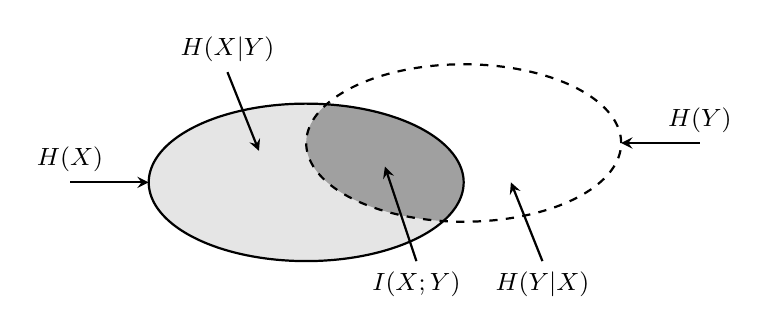
\begin{tikzpicture}[scale=2]
\shorthandoff{>}
% interior H(X) x^2 + 4 y^2 = 1 => y = \pm sqrt(1-x^2)/2
\fill[domain=0:360,samples=200,opacity=.1] plot ({cos(\x)},{.5*sin(\x)});
%
% interior H(Y) (x-1)^2 + 4 (y-1/4)^2 = 1 => y = 1/4 \pm sqrt(1-(x-1)^2)/2
% se cruzan cuando x = 1 \pm sqrt(55)/10 =>
% theta = acos(.5 \pm sqrt(55)/20) para X
% theta = acos(-.5 \pm sqrt(55)/20) para X
\pgfmathsetmacro{\s}{acos(.5-sqrt(55)/20)};
\pgfmathsetmacro{\t}{-acos(.5+sqrt(55)/20)};
\pgfmathsetmacro{\u}{-acos(-.5+sqrt(55)/20)};
\pgfmathsetmacro{\v}{acos(-.5-sqrt(55)/20)-360};
%
% interior I(X;Y)
%\draw[domain=\v:\v] plot ({cos(\x)+1},{.5*sin(\x)+.25}) node{$\bullet$};
\fill[opacity=.3]
   plot [domain=\s:\t,samples=200] ({cos(\x)},{.5*sin(\x)})
-- plot [domain=\u:\v,samples=200] ({cos(\x)+1},{.5*sin(\x)+.25})
-- cycle;
%
% borders H(X) y H(Y)
\draw[domain=0:360,samples=200,thick] plot ({cos(\x)},{.5*sin(\x)});
\draw[dashed,domain=0:360,samples=200,thick] plot ({cos(\x)+1},{.5*sin(\x)+.25});
%
% flechas y flechas condicionales
\draw[thick,>=stealth,<-] (-1,0)--(-1.5,0) node[above]{\small $H(X)$};
\draw[thick,>=stealth,<-] (-.3,.2)--(-.5,.7) node[above]{\small $H(X|Y)$};
%
\draw[thick,>=stealth,<-] (2,.25)--(2.5,.25) node[above]{\small $H(Y)$};
\draw[thick,>=stealth,<-] (1.3,0)--(1.5,-.5) node[below]{\small $H(Y|X)$};
%
\draw[thick,>=stealth,<-] (.5,.1)--(.7,-.5) node[below]{\small $I(X;Y)$};
\end{tikzpicture} \end{center}
%
\leyenda{Diagrama  de Venn: Ilustraci\'on  de la  definici\'on de  la entrop\'ia
  condicional, de la informaci\'on mutua, y de las relaciones entre cada medida.
  La superficia del  elipse en linea llena (parte grise)  representa $H(X)$ y el
  interior de la  en linea discontinua representa $H(Y)$.   La parte grise clara
  representa $H(X|Y)$  superficia del ``conjunto $H(X)$'' quitando  la parte que
  partenece  a  $H(Y)$.  La  parte  blanca  representa  $H(Y|X)$ superficia  del
  ``conjunto $H(Y)$''  quitando la  parte que partenece  a $H(X)$.  La  parte en
  grise oscuro es entonces lo que $X$ e $Y$ comparten, es decir $I(X;Y)$.}
%
\label{fig:SZ:Venn}
\end{figure}

Como se lo va a probar, $I$ es positiva; representa realmente una informaci\'on,
la compartida  entre \ $X$  \ e  \ $Y$: Si  de la incerteza  de $X$ se  quita la
incerteza  de  $X$   una  vez  que  $Y$  es  medida,  lo   que  queda  tiene  la
significaci\'on de la informaci\'on que  estas variables tienen en com\'un. Para
probar la positividad  de $I$, se introduce de manera  m\'as general la noci\'on
de    entrop\'ia   relativa,    conocida   tambi\'en    como    divergencia   de
Kullback-Leibler~\cite{KulLei51, Kul68, CovTho06, Rio07}:
%
\begin{definicion}[Entrop\'ia relativa]\label{def:SZ:entropiarelativa}
  La entrop\'ia  relativa, o divergencia  de una distribuci\'on  de probabilidad
  $q$, con respeco  a una distribuci\'on de referencia  $p$, donde \underline{el
    soporte de  $p$ incluye lo  de $q$}  ($p(x) = 0  \Rightarrow q(x) =  0$), es
  definida como
  %
  \[
  \Dkl[q]{p} = \sum_x q(x) \log \left( \frac{q(x)}{p(x)} \right)
  \]
  %
  o, en su forma diferencial
  %
 \[
 \Dkl[q]{p} = \int_{\Rset^d} q(x) \log \left( \frac{q(x)}{p(x)} \right) \, dx
 \]
  %
 (en este \'ultimo caso, la condici\'on de inclusi\'on del soporte de $q$ dentro
 del de $p$ se  formula como de que $q$ es absolutamebte  continua con respeto a
 $p$)~\footnote{M\'as rigorosamente, en el  caso discreto, esta cantidad depende
   solamente de $p$ y  $q$ y no de los estados. La  condici\'on necesaria es que
   $p$ y $q$  tienen los mismos n\'umeros de componentes  (se completa el vector
   lo m\'as corto) y si la $i$-esima componente de $q$ vale cero, entonces la de
   $p$ vale cero tambi\'en.  Adem\'as, con $p$ y $q$ de mismo tama\~no, se puede
   poner en  biyecci\'on los  alfabetos asociados  a $p$ y  $q$, sin  perdida de
   generalidad.   En el  caso continuo,  esta razonamiento  no vale  m\'as, esta
   cantidad dependiendo de los estados\ldots}.
\end{definicion}
%
Inicialmente, esta  medida fue  introducida por Kullback  y Leibler en  la misma
linea que  Shannon, interpretando \  $\log\left(\frac{q(x)}{p(x)}\right)$ \ como
una informaci\'on de discriminaci\'on  entre dos hip\'otesis de distribuciones \
$q$ \ y \  $p$ \ a partir de la observaci\'on \ $x$,  \ la divergencia siendo la
informaci\'on   de  discriminaci\'on   promedia.   Introdujeron   tambi\'en  una
versi\'on sim\'etrica, que veremos m\'as adelante.

Esta medida puede  ser vista tambi\'en como una  entrop\'ia de la distribuci\'on
$q$, relativamente  a una distribuci\'on de  referencia $p$. Por  ejemplo, en el
caso discreto finito, si $p$ es  la distribuci\'on uniforme sobre un alfabeto de
cardinal  $\alpha$, $\Dkl[q]{p} =  \log \alpha  - H(q)$,  lo que  representa una
desviaci\'on de  la entrop\'ia de  su valor m\'aximo. La  misma interpretaci\'on
queda en  el caso continuo  con la  ley uniforme ($p$  y $q$ definidas  sobre el
mismo espacio de  volumen finito) o con  la gaussiana ($p$ y $q$  dando la misma
matriz de covarianza).  {\it Como para la entrop\'ia,  cuando se necesitar\'a un
  logaritmo   especificamente  de   base   $a$,  se   notar\'a  la   divergencia
  $D_{\mathrm{kl},a}$.}

\begin{lema}[Positividad de la entrop\'ia relativa]
  %
  \[
  \Dkl[q]{p} \ge 0 \quad \mbox{con igualdad ssi} \quad p = q \: (c.s.)
  \]
  %
  donde $(c.s.)$ significa ``casi siempre''.
\end{lema}
%
\begin{proof}
  Existen varias pruebas, pero la m\'as linda puede ser la usando la desigualdad
  de Jensen~\footnote{Se  puede usar tambi\'en  la desigualdad \ $\sum  t_i \log
    t_i \ge \sum t_i \log t'_i$  \ una instancia de la desigualdad conocida como
    desigualdad log-sum, o conocida  tambi\'en como desigualdad de Gibbs (debido
    a   J.  W.   Gibbs   mismo)~\cite{CovTho06,  Rio07,   Gib}.}:  para   $\phi$
  estrictamente convexa, $\Esp[\phi(X)] \ge  \phi(\Esp[X])$ con igualdad ssi $X$
  es  determinista (casi  siempre).  Sea  $X$ de  distribuci\'on  o densidad  de
  probabilidad  $p$.   En el  caso  discreto  como  diferencial, se  escribe  la
  entrop\'ia  relativa $\Dkl[q]{p}  = \Esp\left[  \frac{q(X)}{p(X)}  \log \left(
      \frac{q(X)}{p(X)}  \right)  \right]$.    Sea  $Y  =  \frac{q(X)}{p(X)}$  y
  $\phi(u) = u \log u$, funci\'on estrictamente convexa.  Entonces $\Dkl[q]{p} =
  \Esp[\phi(Y)]   \ge   \phi(\Esp[Y])$.  \   Pero   \   $\Esp[Y]  =   \Esp\left[
    \frac{q(X)}{p(X)} \right]  = \sum_x q(x)  = 1$ \  (y con una integral  en el
  caso diferencial)  y \  $\phi(1) =  0$, lo que  cierra la  prueba. El  caso de
  igualdad  apareciendo  si  y  solamente  si  $Y$  es  determinista,  es  decir
  $\frac{p(X)}{q(X)}$  determinista,  es equivalente  a  $p(x)  \propto q(x)  \:
  (c.s.)$, \ie $p = q \: (c.s.)$ porque ambas suman a uno.
\end{proof}

Esta propiedad, v\'alida en el  caso discreto como continuo, tiene consecuencias
fijandose de que
%
\[
I(X;Y) = \Dkl[p_{X,Y}]{p_X p_Y}
\]
%
\ie  la  informaci\'on  mutua  es  la  divergencia  de  Kullback-Leibler  de  la
distribuci\'on conjunta relativa al producto de las marginales.
%
\begin{propiedades}
\item\label{prop:SZ:Ipositive}   {\it   $I$   es   positiva,  como   medida   de
    independencia:}
  %
  \[
  I(X;Y) \ge 0 \quad \mbox{con igualdad ssi $X$ e $Y$ son independientes}
  \]
%
\item\label{prop:SZ:condicionar} {\it  Condicionar reduce la  entrop\'ia}
  %
  \[
  H(X|Y) \le H(X) \quad \mbox{con igualdad ssi $X$ e $Y$ son independientes}
  \]
  %
  Esta    desigualdad,     con    la     regla    de    cadena,     prueba    la
  sub-aditividad~\ref{prop:SZ:subaditividad}.   Esta  reducci\'on  de  incerteza
  vale en  promedio, pero el conocimiento  de un valor particular  puede ser tal
  que $H(X|Y =  y) > H(X)$, \ie !` un conocimiento  particular puede aumentar la
  entrop\'ia!  (ver ejemplos en~\cite[p.~59]{Rio07}).
\end{propiedades}

Fijense  que   si  $\Dkl{}$  es   positiva,  \underline{no  es   sim\'etrica}  y
\underline{tampoco  satisface la  desigualdad triangular}.  Por eso,  no  es una
distancia  y  tiene  el  nombre  de {\it  divergencia}.   La  distribuci\'on  de
referencia $p$ juega un rol fundamental.

Al  final, a  pesar  de que  la forma  diferencial  de $\Dkl{}$  depende de  los
estados, queda invariante bajo  una misma transformaci\'on biyectiva sobre ambos
$p$ y $q$.
